\RequirePackage{fix-cm}
\documentclass[twocolumn]{svjour3}
\smartqed
\usepackage{amsmath,amssymb,graphicx,booktabs}
\usepackage[numbers,sort&compress]{natbib}
\usepackage[hidelinks]{hyperref}
\providecommand{\bibcommenthead}{}
\providecommand{\burl}[1]{\url{#1}}
\providecommand{\arxivurl}[1]{\url{#1}}
\newenvironment{bchapter}{}{}
\newenvironment{barticle}{}{}
\newenvironment{botherref}{}{}
\newenvironment{bbook}{}{}
\setlength{\emergencystretch}{2em}
\hyphenation{un-known}
\journalname{International Journal of Information Security}
\begin{document}
\title{Legal Label Vocabularies and Attainable Macro F1 in Intrusion Detection Benchmarks}
\titlerunning{Legal vocabularies and attainable macro F1}
\author{Shah Zaib Sajid}
\institute{Shah Zaib Sajid \at Independent Researcher, Rawalpindi, Pakistan\\\email{shahzaibjanjua25@gmail.com}}
\date{}
\maketitle
\begin{abstract}
Intrusion detection benchmarks can ask a classifier to name attack labels outside its legal output vocabulary. A low macro F1 then combines recognition error with a structural evaluation constraint. We formalize a count-based audit for pooled predictions from folds with different legal vocabularies. A coverage bound provides a pre-training check; an exact vocabulary oracle accounts for false positives caused by mandatory predictions. We establish tightness conditions, group optimal allocations by identical vocabularies, and distinguish positive-support, fixed-inventory, and inferred-union scoring. A rational verifier agrees with exhaustive row-level enumeration in 720 comparisons. Benchmark re-scoring reproduces fine-label ceilings of 0.553 on NSL-KDD and 0.067 on CICIDS2017 day holdout. A fresh RT-IoT2022 experiment comprises sixty fits on a fixed, exact-feature-group-separated cohort. Withholding the dominant attack label lowers the exact fine-label oracle from the coverage bound of 0.917 to 0.843, while separately fitted binary detectors retain mean macro F1 of 0.987. A targeted audit of twenty-three studies distinguishes compatible scores, different targets and insufficient information. Eighteen independently re-scored matrices from three studies illustrate metric interpretation, including an unresolved CICIoT2023 summary reconciliation. These results support a reporting contract that declares the target, legal outputs, scoring inventory, oracle status, and operational detection behavior.\keywords{Intrusion detection \and Benchmark evaluation \and Macro F1 \and Label vocabulary \and Reproducibility}\end{abstract}
\section{Introduction}
An intrusion detector may fail to identify an attack because the features do not distinguish it, because the training procedure learns a poor boundary, or because its prediction interface cannot emit the required label. The last failure is structural. Increasing training time cannot create an output that the classifier is forbidden to use. Yet these causes can contribute to the same reported classification score.

Consider the official NSL-KDD partition. Its test data contain 38 fine-grained labels, of which 21 occur in training. A classifier whose outputs are restricted to observed training labels cannot correctly name the other 17 labels. If evaluation averages F1 over all 38 test-positive labels, its score cannot exceed 21/38 even under otherwise perfect decisions. Mapping the task to five broad categories removes this particular restriction, but changes the question from subtype attribution to category recognition. Neither score replaces the other.

This distinction matters when interpreting experiments involving unknown attacks. A binary detector may correctly alarm on a previously unseen attack subtype because ATTACK remains a legal output. A classifier asked to assign the subtype's exact name faces a different task. Open-set rejection and zero-shot attribution create still other output contracts. Absence from training is therefore evidence of an output constraint only when the prediction vocabulary actually excludes that label.

Security evaluation already has a substantial literature on experimental bias and operational relevance \cite{sommer2010} \cite{arp2022}. The contribution here is narrower: a reproducible audit that connects fold-level label counts, legal decisions, and the exact definition of pooled macro F1. The elementary coverage inequality is a scoring corollary, not a new theory of F1. The stronger mathematical component concerns attaining that inequality when every test row must be routed to a legal label.

We address three questions. \textbf{RQ1:} Which pooled scores are possible under declared fold-specific vocabularies, and when is a simple coverage bound tight? \textbf{RQ2:} How do output inventories and target resolution affect attainable scores and detection behavior? \textbf{RQ3:} What can be checked in published evaluations when methodological details or confusion counts are available? The artifact supplies a count interface, two floating-point solvers, an independent rational verifier, saved confusion matrices, fresh matched-preprocessing refits, and source-level audit records. We separate numerical reproduction from source interpretation throughout.

\section{Related work and scope}
Metric choice is part of the evaluation target. Opitz and Burst distinguish two formulas commonly called macro F1: the average of classwise F1 and the harmonic mean of macro precision and recall \cite{opitzburst2019}. Opitz analyzes metric behavior under prevalence and prediction bias \cite{opitz2024}. Forman and Scholz show that aggregation choices in cross-validation can invalidate apparently comparable performance summaries \cite{forman2010}. We use the arithmetic mean of classwise F1 after pooling confusion counts. Averaging fold scores is a separate objective.

Balikas et al. derive performance bounds for regularized model selection using unlabeled samples, estimated class priors and quantification assumptions \cite{balikas2015}. Their F1-related bounds are probabilistic under an IID sampling model. Our oracle is instead a deterministic maximum over row decisions for a fixed labeled cohort with fold-dependent legal outputs. The existence of F1 bounds is prior work; the present derivation concerns this particular feasible set and its mandatory destination loss.

Optimization over confusion matrices is also established. Narasimhan et al. develop consistent learning algorithms for complex multiclass performance measures \cite{narasimhan2015}. Our feasible set instead fixes the test labels and legal fold outputs and permits arbitrary row-level decisions. The resulting maximum is a diagnostic of the evaluation contract. It does not describe a trainable model or optimize a deployment policy.

Open-set recognition permits unfamiliar inputs to be assigned an unknown decision \cite{scheirer2013}. Zero-shot recognition may name unseen semantic classes using side information \cite{xian2017}. Such models cannot automatically be assigned the training-restricted vocabulary used in a conventional tree classifier. Similarly, TESSERACT addresses temporal and spatial biases in malware evaluation \cite{pendlebury2019}; a unit label-coverage bound does not establish that these biases are absent. CICIDS2017 audits identify feature-extraction and labeling defects that require separate treatment \cite{engelen2021} \cite{lanvin2023}.

Cruz et al. already distinguish fine exploit recognition from coarse families and binary detection, and introduce an explicit unknown decision \cite{cruz2017}. Their evaluation uses accuracy and a cost-of-unknown analysis. We do not claim that the distinction between naming an unseen attack and detecting it is new. The grouped oracle supplies a count-conditioned limit for pooled macro F1 under a declared prediction contract.

Recent IDS studies already recognize parts of this distinction. Reis explicitly uses a binary target to avoid unresolved multiclass label-coverage issues under scenario-aware splitting \cite{reis2026}. CLAIRE evaluates class-label coverage in active-learning selection \cite{almalawi2025}. Its selection coverage concerns which classes receive annotations, whereas our quantity measures the fraction of each class's test rows whose true label is legal in the relevant fold. These connections motivate an audit interface; they do not establish priority for the basic coverage observation. The targeted search found no equivalent grouped oracle in the inspected sources, but is insufficient to prove that none exists.

\section{Evaluation contract and coverage}
Let $f$ index folds, $T_f$ be the observed training-label set, and $V_f$ be the nonempty legal output vocabulary for each nonempty test fold. Each test row receives exactly one prediction in $V_f$. Labels are mutually exclusive, and a pooled test row is counted once. Let $n_{f k}$ denote the number of test rows with true label $k$ in fold $f$. Define
\begin{equation}\begin{aligned}S&=\{k:\sum_f n_{fk}>0\},\quad n_k=\sum_f n_{fk},\\m_k&=\sum_f n_{fk}\mathbf1\{k\in V_f\}.\end{aligned}\end{equation}
For $k \in S$, the covered fraction is $\rho_k=m_k/n_k$. Training-restricted classifiers satisfy $V_f=T_f$, but the interface accepts explicit $V_f$ rather than imposing that equality. Training-only and other output-only labels must remain in the input even when their test support is zero.

With false positives $\mathrm{FP}_k$ and true positives $\mathrm{TP}_k$, classwise F1 is $2\mathrm{TP}_k/(n_k+\mathrm{TP}_k+\mathrm{FP}_k)$. We set undefined zero-support terms to zero. The primary score averages over $S$. A fixed global inventory $R$ is also allowed, provided $S \subseteq R$; its extra zero-support labels remain in the denominator. An inferred-union scorer instead adds only output-only labels actually predicted. These conventions must not be silently interchanged.

\textbf{Proposition 1 (coverage bound).} Every legal prediction vector satisfies
\begin{equation}F_S\le C_S=\frac1{|S|}\sum_{k\in S}\frac{2m_k}{n_k+m_k}=\frac1{|S|}\sum_{k\in S}\frac{2\rho_k}{1+\rho_k}.\end{equation}
\textbf{Proof.} A correct prediction requires a legal true label, so $\mathrm{TP}_k\le m_k$. The classwise F1 expression increases with true positives and decreases with false positives. Substituting $m_k$ for true positives and zero for false positives proves the result. Classes with $m_k=0$ contribute zero. $\square$

For a fixed inventory, $C_R=C_S |S|/|R|$. Support-weighted F1 has bound $\frac{\sum_{k\in S}n_k\frac{2m_k}{n_k+m_k}}{\sum_k n_k}$. When all true and predicted labels are included, micro F1 equals accuracy and has the \textbf{attainable} ceiling $\frac{\sum_k m_k}{\sum_k n_k}$. Balanced accuracy has attainable ceiling $\frac{\sum_{k\in S}\rho_k}{|S|}$. Repairing every available row attains the last two ceilings, regardless of the destinations of unavailable rows. The macro-F1 bound need not be attainable because those destinations can add false positives to contributing classes.

If a label appears in exactly one group in leave-one-group-out evaluation using all remaining groups as training, its covered fraction is zero. If it appears in at least two groups, its covered fraction is one. Fractional pooled coverage therefore requires a different structure, such as forward chaining or a restricted training window. A global output head containing all test labels has $C_S=1$ even without training examples of every label. This bound concerns output legality, not learnability.

\section{Exact attainable score}
Correcting an error on an available row cannot reduce macro F1. It increases that class's true positives and removes a false positive from the previous destination. For inferred-union scoring it also cannot introduce a new label into the denominator, since the corrected label already has true support. Thus an optimum may be taken to classify all available rows correctly.

Let $U_f=\sum_\{k \notin V_f\} n_{f k}$ be the unavailable mass in fold $f$. Write $a_{f k}$ for its allocation to legal destination $k$, with $a_{f k}\ge 0$, $a_{f k}=0$ outside $V_f$, and $\sum_k a_{f k}=U_f$. Let $a_k=\sum_f a_{f k}$. The support-scored vocabulary oracle is
\begin{equation}O_S=\max_a\frac1{|S|}\sum_{k\in S}\frac{2m_k}{n_k+m_k+a_k}.\end{equation}
This maximum permits decisions that depend on true test labels. It is an upper limit for a declared cohort and vocabulary, not an executable detector.

\subsection{Vertex allocation and equality}
\textbf{Theorem 1 (vertex allocation).} An optimum sends all unavailable rows of each fold to one legal destination.

\textbf{Proof.} For $m_k>0$, the second derivative of the score term with respect to $a_k$ is $4m_k/(n_k+m_k+a_k)^3>0$; other terms are constant. The objective is convex on the product of allocation simplexes. Every feasible point is a convex combination of vertices, so at least one vertex has score no smaller. Vertices route each fold's entire mass to one destination and are integer feasible. Combined with the repair argument, this proves attainability of an optimum over actual row predictions. $\square$

\textbf{Theorem 2 (tightness).} Under support or fixed-inventory scoring, $O=C$ if and only if every fold with $U_f>0$ permits at least one destination $k$ with $m_k=0$. A destination outside $S$ automatically satisfies this condition.

\textbf{Proof.} Sending unavailable rows only to such destinations adds no false positives to a positive-numerator term, so it attains $C$. Conversely, if a fold permits only positive-$m_k$ destinations, its positive unavailable mass necessarily enters at least one strictly decreasing term. The finite set of integer row allocations then has maximum strictly below $C$; Theorem 1 justifies restricting the displayed continuous simplex to such vertices. $\square$

For example, take one fold with true labels A, B, C and legal outputs A, B. The coverage bound is $2/3$. Repairing A and B leaves C to be predicted as either A or B. The best score is $(2/3+1+0)/3=5/9$. The gap $1/9$ is mandatory false-positive loss, not learning error. If an output-only label D is permitted, support scoring attains $2/3$ by routing C to D. A fixed inventory containing D still scores its zero term, and inferred-union scoring charges D only when activated.

\subsection{Grouping, limits, and certificates}
If no fold has unavailable mass, the destination union is empty ($q=0$) and $O=C$ without enumeration.
Folds with identical legal vocabularies can be grouped by summing their unavailable masses. Their feasible aggregate allocations form a simplex with that summed mass; Theorem 1 applies again. If the union of destination labels in unavailable folds has size $q\ge 1$, the number of grouped vertex choices is bounded by
\begin{equation}\prod_{j=1}^q j^{\binom qj}\le q^{2^q-1}.\end{equation}
This yields an exact algorithm parameterized by $q$, with polynomial arithmetic work per candidate. It does not promise practical performance for large $q$. A Set Cover reduction in the supplementary material establishes worst-case NP-hardness for arbitrary vocabularies. Enumeration and branch-and-bound must report when a resource budget prevents certification.

For quick bounds, define the unaveraged destination loss $g_k(a)=2m_k/(n_k+m_k)-2m_k/(n_k+m_k+a)$ and set it to zero outside $S$. Let $c_f=\min_\{k \in V_f\} g_k(U_f)/|S|$. Monotonicity and concavity of each loss function give
\begin{equation}\max(0,C_S-\sum_f c_f)\le O_S\le C_S-\max_f c_f.\end{equation}
Routing each fold to its individual minimum-loss destination gives the lower bound, using subadditivity of $g_k$. Any complete allocation loses at least each fold's isolated minimum, giving the upper bound. These polynomial bounds remain available when exact search is too expensive.

Under inferred-union scoring, the denominator becomes $|S|+|W|$, where $W=\{k \notin S:a_k>0\}$. Vertex allocation and grouping remain valid: restrict decisions to the outside labels used by an optimum, maximize the convex numerator at a vertex, and observe that dropping outside outputs cannot worsen the denominator. If $C_S>0$, equality with $C_S$ additionally requires no outside output to be activated; every unavailable fold must have a legal zero-$m_k$ destination within $S$. If $C_S=0$, equality is automatic. The software checks this boundary case explicitly.

The independent verifier enumerates grouped vertices using rational arithmetic and returns an exact fraction, per-class false-positive totals, and one destination for each unavailable fold. Reconstructing the repaired prediction vector verifies feasibility and its score. Exhaustion of the vertex set certifies optimality; a witness alone certifies only a feasible lower bound. This distinction is essential for interpreting time-limited optimization outputs.

\section{Experimental methods}
We distinguish three kinds of evidence: re-scoring saved benchmark predictions; fresh model training from downloaded data; and source-based interpretation of published evaluations. No test label is used for feature selection, fitting, or tuning. The truth-dependent oracle is computed only for auditing. Synthetic enumeration tests are reported separately from traffic experiments.

\subsection{Benchmark evidence and fresh refits}
The released artifact contains aggregate counts and saved predictions for original-label NSL-KDD \cite{tavallaee2009} and CICIDS2017 \cite{sharafaldin2018}, corrected CICIDS2017, and supplementary controls. We regenerate the principal tables from confusion counts and verify the existing fit records. The corrected-release experiment is an earlier saved run, not a newly trained result in this revision. Source hashes and split manifests are retained; raw traffic is not redistributed here.

For a fresh check, we downloaded the public NSL-KDD training and test files from a documented mirror and retained their SHA-256 hashes. The official split has 125,973 training rows and 22,544 test rows. Features comprise the first 41 fields; neither class nor difficulty enters fitting. Random Forest and Extra Trees use the same training-fitted one-hot encoding for the three nominal fields, numeric passthrough, 200 trees, minimum leaf size two, and minimum split size five. Seeds 42--44 are fixed before execution. Saved arrays retain truth, predictions, labels, and confusion counts. Exact feature overlap and duplicate counts are checked and recorded in the run manifest. The analysis compares two complete pipelines with matched preprocessing; three seeds on one cohort quantify fitting variation only.

The paired resolution analysis maps both truth and predictions to the declared five-category NSL taxonomy without refitting. It answers whether the \textbf{same decisions} receive different scores when their semantic resolution changes. It does not estimate the result of training a separate category-level model. The original CICIDS2017 comparison uses pooled five-fold stratified CV versus capture-day holdout. Its CSV release lacks timestamps, so a historical within-day row-order analysis is excluded from temporal conclusions. The corrected-release experiment instead trains on Monday through Thursday and tests Friday, with three models and three seeds at a 5,000-per-class training cap.

The duplicate audit finds 654 distinct feature vectors shared by the official partitions. A separate control removes all 658 training rows with those vectors and refits the same six settings on 125,315 training rows, retaining the full test cohort. Removal uses exact feature identity, without test labels; it is a split-hygiene control informed by test features, not a prospective deployment procedure. There is no exact feature overlap after removal. Within-training and within-test repetitions remain recorded, and session-level dependence is not eliminated by this check.

\subsection{RT-IoT2022 vocabulary intervention}
We add a fresh traffic-data experiment using the UCI RT-IoT2022 release \cite{rtiot2024}. Its downloaded file contains 123,117 rows, twelve fine labels, including three benign device-activity labels. We remove the row index and both port columns, leaving 81 inputs. Exact identity on these inputs gives 18,272 groups, with no hash collisions against direct duplicate elimination. The first fold of five shuffled stratified group folds (seed 20261115) supplies 31,061 test rows; all twelve labels occur on both sides and no exact input vector crosses the split. This is a feature-group holdout, not a temporal or device-independent deployment test.

The locally recorded plan precedes model fitting but follows dataset inspection. We evaluate all nine single-attack-label omissions and an all-label baseline on the same test cohort. For each of seeds 42--44, at most 1,000 training rows per original fine label are sampled once; an omission removes only that label's sampled rows. Each condition fits a fine-label attribution task and a separate binary target on identical remaining rows. Extra Trees uses 100 trees and minimum leaf size two; training-fitted median imputation and categorical one-hot encoding precede both fits. All 60 fits have saved predictions, confusion counts, and source-row memberships. Seed variation includes training subsampling and fitting; it does not provide population uncertainty.

\subsection{Published-source audit}
The earlier frozen Crossref screen contains 50 sampled candidates from a 385-record title-filtered frame: three eligible, fourteen excluded, and thirty-three unresolved. We preserve that screen and do not recode it on the basis of later targeted searches. The revision adds a targeted, non-probability source audit, recording queries, retrieval date, DOI, target resolution, legal outputs, metric convention, and the limits of each conclusion. Numerical re-scoring covers ten saved matrices from Franco-Valiente et al., two displayed matrices from Neto et al., and six binary matrices in the author manuscript of the Bot-IoT study \cite{francovaliente2026} \cite{neto2023} \cite{koroniotis2019}. These are three studies, not eighteen independent studies. Author-manuscript and journal-version evidence are distinguished.

For CICIoT2023, all 128 integer cells were transcribed from publisher HTML and automatically checked against Tables 7 and 8 of the publisher PDF. The analysis recomputes classwise F1, macro F1, support-weighted F1, and accuracy. Every class has nonzero true positives, demonstrating its availability in the evaluated decisions. This makes the legal-output ceiling one for the displayed eight-class setting. Training counts, raw split membership, and exact agreement between the summary and matrix-generating runs are not reconstructed.

\section{Results}
\subsection{Coverage, target resolution, and fresh replication}
The original NSL-KDD test set has 3,750 rows with labels absent from training. The support-scored coverage bound and exact oracle are both 21/38, or 0.553. Output-only training labels provide cost-free destinations under support scoring. Under inferred-union scoring, activating those labels enlarges the denominator, and the oracle falls to 0.548. The distinction is small here but follows from the metric contract, rather than a change in predictions.

The five previously released forest matrices give mean fine-label F1 0.240 (sample SD 0.009). Mapping those same matrices to five categories gives 0.483 (SD 0.005), with ceiling one. Every attack family contains a test-only subtype, so an internally consistent mapping that groups all such families reduces to this same five-category target. Grouping only selected true rows while leaving sibling predictions fine-grained would not define a common taxonomy.

\begin{table*}[t]
\caption{Fresh NSL-KDD fits with matched preprocessing. Mean macro F1 (sample SD) over seeds 42--44; all six fits share the official test cohort. Fine support ceiling 0.553; five-category ceiling one.}\label{tab-nsl}
\centering\small
\begin{tabular}{llll}\toprule
Pipeline & Fine / support & Fine / union & Five categories\\
\midrule
Random Forest & 0.242 (0.011) & 0.236 (0.010) & 0.482 (0.007)\\
Extra Trees & 0.224 (0.001) & 0.218 (0.001) & 0.481 (0.004)\\
\bottomrule\end{tabular}
\end{table*}


Table~\ref{tab-nsl} reports the fresh matched-preprocessing fits. Forest seeds 42 and 43 reproduce the released fine-label scores to numerical precision; the machine-readable comparison checks all three seeds. Both estimators have zero true positives on unavailable fine labels. The coarse projection raises their scores without creating correct subtype predictions. This demonstrates the interpretive effect directly while controlling preprocessing between these two pipelines. It does not establish a population-level estimator ranking.

\begin{table*}[t]
\caption{NSL-KDD overlap-controlled refits: 658 training rows removed by exact feature identity, full test cohort retained. Mean macro F1 (sample SD) across three seeds. Vocabulary ceilings are unchanged.}\label{tab-overlap}
\centering\small
\begin{tabular}{llll}\toprule
Pipeline & Fine / support & Fine / union & Five categories\\
\midrule
Random Forest & 0.239 (0.013) & 0.233 (0.013) & 0.483 (0.001)\\
Extra Trees & 0.223 (0.001) & 0.217 (0.001) & 0.483 (0.003)\\
\bottomrule\end{tabular}
\end{table*}


Table~\ref{tab-overlap} gives the refit after training-row overlap removal. Both legal label inventories remain unchanged, and the fine-label ceiling stays at 21/38. Scores change modestly while zero attribution recall on unavailable labels persists. The official-split replication therefore contains an additional feature-overlap concern, but the coverage result survives the control. This demonstrates why legal-output auditing and duplicate checks should be reported together.

\subsection{CICIDS2017: attribution and detection separate}
In the original five-day holdout, each of the fourteen fine-grained attack labels occurs on one day only. BENIGN remains available. Thus all attack F1 terms are fixed at zero, the support-scored ceiling and oracle are 1/15, and a classifier's fine-label score is exactly benign F1 divided by fifteen. The archived unweighted forest scores 0.853 in shuffled CV and 0.060 in day holdout. These protocols address different generalization questions; subtracting their scores does not isolate one cause of failure.

The day-holdout score reaches 90.5\% of its ceiling while detecting only 14.7\% of attack rows after binary projection. Predictions assigned to incorrect attack labels still count as binary alarms, whereas predictions assigned to BENIGN miss the attack. Consequently high ceiling attainment can coexist with poor attack detection. The projected binary macro F1 is 0.580 under a unit legal ceiling. A separately trained binary forest is another experiment, with its own saved result and training target.

The corrected CICIDS2017 Friday cohort has five test-positive labels, of which only BENIGN occurs in Monday--Thursday training. Its fine-label ceiling is 0.200. The earlier nine fits yield mean fine-label F1 of 0.155 for Random Forest, 0.155 for Extra Trees, and 0.175 for SGD. Binary attack recalls are 0.359, 0.361, and 0.807, respectively. The training cap changes priors and model settings differ; these values illustrate target interpretation rather than an isolated effect of label correction or a definitive model comparison.

\begin{table*}[t]
\caption{Original CICIDS2017 day-holdout predictions mapped to three targets. All rows re-score the same pooled predictions, without refitting.}\label{tab-target}
\centering\small
\begin{tabular}{llll}\toprule
Target & Classes & Coverage bound & Macro F1\\
\midrule
fine attack label & 15 & 0.067 & 0.060\\
eight-family mapping & 8 & 0.250 & 0.156\\
binary benign/attack & 2 & 1.000 & 0.580\\
\bottomrule\end{tabular}
\end{table*}


\begin{figure*}[t]\centering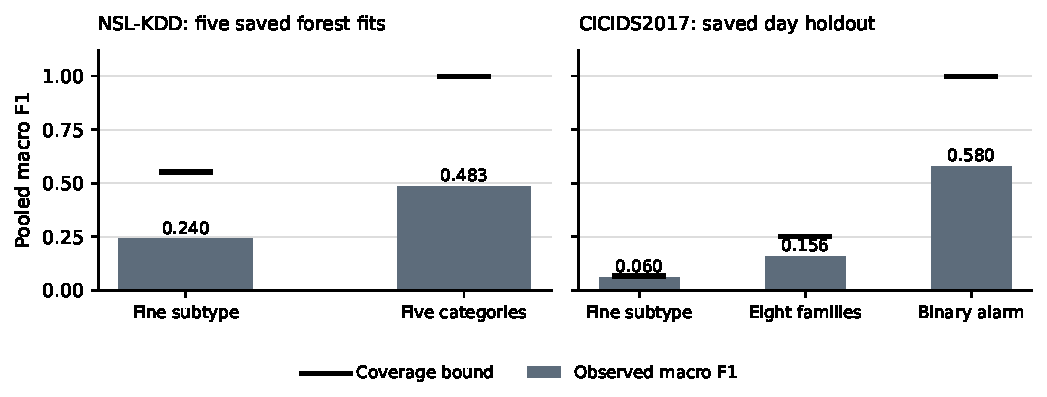
\includegraphics[width=\textwidth]{target_resolution.pdf}\caption{Changing target resolution changes both the observed score and its coverage bound. Within each panel the predictions are fixed; the targets differ. NSL values are means over five saved fits. These bars do not compare model quality across tasks.}\label{fig-target}\end{figure*}

Fig.~\ref{fig-target} summarizes the paired changes. In each dataset, a higher score at coarser resolution must be interpreted with its newly defined target and ceiling.

\subsection{Exactness checks and unavoidable destination loss}
The original implementation checks pass on 80 row-level inputs under both support and union scoring, with another 100 cases using explicit heads. The new independent rational verifier adds 240 inputs, each evaluated under support, union, and fixed scoring: 720 exact comparisons against unrestricted row-level enumeration. It verifies returned routing witnesses and tightness decisions, and checks zero coverage, output-only labels, invalid inputs, large integer counts, and resource budgets. The tests share input preparation with the production solver, so input validation also has dedicated adversarial checks.

The minimal all-cost example gives $C=2/3$ and $O=5/9$ exactly. In the released fractional-coverage digits control, the coverage bound is 0.950 and the oracle is 0.922. This is a deliberately constructed protocol on real digit data, not a traffic benchmark. The supplementary gas-drift example has a smaller gap, 0.012. These contrasts show that the analytical bound can be loose, but the size and practical importance of that correction depend on the cohort. Large synthetic oracle problems can exhaust their search budgets; such runs remain uncertified.

\subsection{RT-IoT2022: a controlled vocabulary intervention}
\begin{table*}[t]
\caption{RT-IoT2022 feature-group holdout: 31,061 fixed test rows with no identical input vector shared with training. F1 is macro F1, shown as mean (sample SD) over three seeds. Held alarm recall is the separately fitted binary detector's mean recall on the withheld subtype. Fine and binary fits share capped training rows; NONE retains all labels. These are dependent variants on one cohort.}\label{tab-rt}
\centering\small
\begin{tabular}{llllll}\toprule
Withheld label & Bound & Oracle & Fine F1 & Binary F1 & Held alarm recall\\
\midrule
NONE & 1.000 & 1.000 & 0.847 (0.004) & 0.984 (0.000) & --\\
ARP poisioning & 0.917 & 0.914 & 0.666 (0.019) & 0.884 (0.012) & 0.164\\
DDOS Slowloris & 0.917 & 0.916 & 0.780 (0.005) & 0.984 (0.000) & 1.000\\
DOS SYN Hping & 0.917 & 0.843 & 0.679 (0.008) & 0.987 (0.006) & 1.000\\
Metasploit Brute Force SSH & 0.917 & 0.917 & 0.766 (0.002) & 0.987 (0.006) & 1.000\\
NMAP FIN SCAN & 0.917 & 0.917 & 0.850 (0.001) & 0.984 (0.000) & 1.000\\
NMAP OS DETECTION & 0.917 & 0.916 & 0.712 (0.023) & 0.987 (0.005) & 1.000\\
NMAP TCP scan & 0.917 & 0.916 & 0.723 (0.004) & 0.984 (0.000) & 1.000\\
NMAP UDP SCAN & 0.917 & 0.917 & 0.789 (0.001) & 0.980 (0.000) & 0.574\\
NMAP XMAS TREE SCAN & 0.917 & 0.916 & 0.735 (0.008) & 0.990 (0.005) & 1.000\\
\bottomrule\end{tabular}
\end{table*}


With all labels available the bound and oracle equal one. Every omitted label instead fixes the simple bound at 11/12, but the mandatory false positives lower the exact oracle. Omitting DOS SYN Hping, which accounts for 25,894 test rows, gives an oracle of 0.842606, a gap of 0.074061 below the bound. Thus the exact correction has a material effect on a traffic-data cohort, beyond the constructed digits control. The fine classifier cannot name the withheld label, whereas the binary classifier retains both legal outputs. Its mean macro F1 is 0.987 for this omission. This result separates a guaranteed attribution failure from empirical detection behavior; it does not imply that all unseen attacks are detected.

Omitting ARP poisoning lowers mean binary macro F1 to about 0.884, despite its unit binary ceiling. The FIN-scan class has one test row, preventing a stable class-specific generalization claim. For ARP poisoning, mean withheld-label alarm recall is only 0.164, despite overall attack recall of 0.954; UDP-scan withheld alarm recall is 0.574. Aggregate binary F1 therefore cannot certify detection of the omitted subtype. Strong duplicate concentration and laboratory conditions further limit external validity. An independent verifier reconstructs all sixty confusion matrices and scores, verifies matched memberships and feature-group separation, and independently enumerates destinations for all thirty fine-label oracles.

\subsection{Published evaluations and matrix reconciliation}
Franco-Valiente et al.'s ten connection-grouped CICIDS2017 matrices reproduce mean macro F1 0.900, agreeing with the published mean; all five evaluated classes have training support \cite{francovaliente2026}. Their legal-output ceiling is one. This check verifies the released artifact's metric arithmetic, rather than reproducing distributed training.

\begin{table*}[t]
\caption{CICIoT2023 eight-class F1 computed from published Tables 7 and 8 versus the corresponding Table 6 entry. Both matrices contain 10,340,161 observations. Summary reconciliation is unresolved; these are not ceiling violations.}\label{tab-external}
\centering\small
\begin{tabular}{llll}\toprule
Model & Matrix macro F1 & Summary F1 & Absolute gap\\
\midrule
DNN & 0.70495 & 0.69726 & 0.00769\\
RF & 0.71958 & 0.71929 & 0.00029\\
\bottomrule\end{tabular}
\end{table*}


For the more recent CICIoT2023 benchmark, Table~\ref{tab-external} compares the matrix-derived macro F1 with the paper's eight-class summary values. The differences are approximately 0.00769 for the neural network and 0.00029 for the forest. Recomputed accuracies also differ slightly from the corresponding summary entries. These discrepancies exceed numerical rounding of the printed F1 values. They establish that the displayed matrices do not exactly reproduce those summary numbers under the stated arithmetic-mean convention. They do not identify which artifact is wrong: the source does not fully connect the displayed matrices to the summary-generating run, and its F1 equation does not explicitly specify multiclass averaging. Both results remain well below a unit legal ceiling. We therefore retain \textbf{verified compatible} for attainability and \textbf{unresolved} for summary-to-matrix reconciliation.

Targeted methods checks reinforce the importance of task resolution. Ayantayo et al. map NSL-KDD to five categories \cite{ayantayo2023}. Biyouki et al. define CICIDS2017 metrics as binary unless stated otherwise, so their leave-one-family-out score of 0.9855 cannot be compared to a fifteen-label attribution ceiling \cite{biyouki2026}. Alsaadi et al. explicitly label their 0.619 whole-day result as binary \cite{alsaadi2026}. Yang et al.'s day-holdout results are also binary \cite{yang2026}, and Reis explicitly declines to base its claims on multiclass scenario-shift results \cite{reis2026}. These are source-based interpretations, not independently re-scored predictions. None establishes an incompatible published score. The expanded targeted ledger contains twenty-three distinct studies: nineteen journal articles, three conference papers and one preprint. It includes established anomaly detectors and explicit-unknown models to test the boundary of applicability. Twenty published studies support a target-level classification; two further published records retain insufficient information, and the preprint is not counted as a published evaluation. These are source audits, not twenty independent model reproductions, and cannot estimate field prevalence.

The Bot-IoT study provides a complementary imbalance check \cite{koroniotis2019}. We transcribe six binary confusion matrices from Tables 10--12 of its author-manuscript version and verify all twenty-four cells against that PDF. For its full-feature SVM, accuracy is 0.999887, while our derived two-class macro F1 is 0.618271: normal-class F1 is 0.236599 and attack-class F1 is 0.999944. Both labels are legal, so its ceiling is one. This is not a claim that the source misreported macro F1; its table uses other metrics. It illustrates why the reporting contract requires the metric definition and classwise behavior even when the vocabulary diagnostic finds no restriction. Journal-PDF identity and original model training are not independently verified.

\section{A reporting contract for IDS benchmarks}
A usable audit begins with the operational decision. Binary alarms, known-family recognition, exact subtype attribution, and scored unknown rejection should be named separately. Next preserve the cohort and fold membership, declare each fold's legal outputs, and record training and test support at the same semantic resolution. A global head must be declared even when some of its outputs lack training examples.

The score definition then states whether predictions are pooled, which labels enter the denominator, and how absent-class terms are handled. Compute the coverage bound before fitting. If mandatory destinations make tightness fail, report the oracle or certified bounds, together with solver status. Report the absolute model score, per-class recall, and binary detection behavior where relevant. A ratio to the oracle can describe attainment on the same cohort, but cannot normalize different targets or datasets into a common model-quality scale.

This sequence can change an experimental decision before training. If an intended unknown-attack study has a training-restricted subtype head with zero coverage for every held-out attack, exact subtype F1 cannot measure its desired detection capability. The researcher can retain the split and report a binary alarm or scored unknown task, or explicitly declare the structural subtype limitation. Changing to a shuffled split merely to raise coverage would also change the generalization question and should not be presented as repairing temporal validity.

\section{Threats to validity}
The bounds condition on trusted labels and declared legal outputs. Incorrect labels, feature leakage, duplicated sessions, and unrealistic traffic remain separate problems. An incorrect vocabulary declaration can make the audit itself misleading. Counts cannot reveal whether a global label is learnable, and a unit ceiling is not a quality certificate.

The fitted evidence uses laboratory benchmarks, including one fresh RT-IoT2022 feature-group holdout. The new NSL refits are on one fixed official partition and three seeds. Shared test rows prevent treating seed results, protocol variants, or model pipelines as independent network observations. We report descriptive means and sample SDs, without significance tests or population confidence intervals. Corrected and original CICIDS2017 results do not form a matched relabeling experiment. The modern CICIoT2023 extension re-scores published counts; its raw model training was not reproduced.

The literature work is a single-agent targeted audit alongside a preserved screening pilot. Search coverage is incomplete, many candidate studies lack enough detail, and no incompatible published score is verified. The CICIoT2023 reconciliation issue remains unresolved without author or artifact clarification. We do not infer misconduct, prevalence, or a failure of its output vocabulary from that mismatch. The rational verifier improves arithmetic assurance, but its grouping argument relies on the proved feasible-set model. Solver validation and manuscript checks were performed by the same automated workflow, not by an independent human replication team.

\section{Conclusion}
Legal output vocabularies impose deterministic limits on pooled classification scores. A simple coverage bound detects missing outputs; mandatory false-positive routing determines whether that bound is attainable. Making both quantities explicit separates exact attack attribution from binary detection and avoids treating changes of taxonomy as improvements to a fixed model. The released implementation combines count-based bounds, grouped optimization, and rational routing certificates. Benchmark re-scoring and fresh refits support the reporting contract, while the published-source audit establishes compatible results and an unresolved matrix reconciliation issue. These findings justify a focused evaluation diagnostic, while operational generalization and broader field prevalence remain open.

\section{Statements and declarations}
\textbf{Funding and competing interests.} The original manuscript declares no research funding and no financial or non-financial competing interests; those declarations are retained.

\textbf{Author contributions.} Shah Zaib Sajid is the sole named author and is responsible for the study and any submission. Generative AI is not an author.

\textbf{Data and code availability.} The repository at \href{https://github.com/shahzaibjanjua25/ids-benchmark-precision-collapse}{github.com/shahzaibjanjua25/ids-benchmark-precision-collapse} contains the original artifact. This revision is supplied as a committed Git branch and self-contained bundle. Its evidence map records commands, data hashes, results, and checks. Public benchmark owners retain their data terms. No raw network traffic is redistributed in this revision. The NSL download mirror and publisher PDF checksum are recorded in manifests.

\textbf{Ethics.} This analysis uses public benchmark files and published aggregate results and performs no traffic collection, human recruitment, or live-system intrusion.

\textbf{Generative AI assistance.} An OpenAI Codex agent assisted research planning, code development, proof checking, source screening, numerical analysis, and manuscript generation. Computations described as executed have corresponding scripts and outputs. Automated review passes do not constitute external peer review. The author must review and take responsibility for any submitted version.

\begingroup\small\bibliographystyle{sn-mathphys-num}\bibliography{references}\endgroup\end{document}